Supppose we have
\begin{itemize}
	\item counter-constant columns $\sourceOne{}, \sourceTwo{}, \target{}, \target{}\new$,
	\item counter-constant columns $\source{}\mark{}, \target{}\mark{}$,
	\item counter-constant column $\size{}$,
	\item binary columns $\bit{1}, \bit{2}, \bit{3}, \bit{4}$
	\item byte columns $\sourceOne{}\byte{}, \sourceTwo{}\byte{}, \target{}\byte{}$,
	\item ``accumulator columns'' $\acc{1}$, $\acc{2}$, $\acc{3}$
	\item some ``power'' column $\col{P1}, \col{P2}$,
	\item a ``counter column'' \ct{}.
	%\item[\vspace{\fill}]
\end{itemize}
%\end{multicols}
The interpreation is as follows:
\sourceOne{}, \sourceTwo{} are limbs from which we will harvest a suffix and a prefix respectively;
\sourceOne{}\byte{}, \sourceTwo{}\byte{}, \target{}\byte{} are the respective byte decompositions of \sourceOne{}, \sourceTwo{} and \target{};
\acc{1} and \acc{2} accumulate the bytes of the desired suffix (of the first source) and prefix (of the second source);
\acc{3} accumulates the bytes of the chunk to isolate (from the target);
$\target{}\new$ is a limb which we will construct the previously extracted suffix and prefix;
\source{}\mark{} is a marker for bytes in \sourceOne{};
\target{}\mark{} is a marker for bytes in \target{};
$\bit{1}$ plateaus at \source{}\mark{};
$\bit{2}$ plateaus at $\source{}\mark{} + \size{} - \llarge$;
$\bit{3}$ plateaus at \target{}\mark{};
$\bit{4}$ plateaus at $\target{}\mark{} + \size{}$;
$\col{P1}$ is pegged to $\bit{4}$ and builds a power of $256$: it is used to left shift the isolate chunk extracted from \target{} and the concatenation of the suffix (of the first source) and prefix (of the second source);
$\col{P2}$ is used concatenate the suffix from \sourceOne{} and the prefix from \sourceTwo{}. 

The following collection of constraints ensures the desired behaviour.
% The interpreation of the greek letters ($\alpha'$, $\beta$) is given in \ob{TODO: add figure}.
\begin{enumerate}
	\item binary plateau constraints:
	\begin{enumerate}
		\item $\plateau(\bit{1}, \source{}\mark{};\ct{})$,
		\item $\plateau(\bit{2}, \source{}\mark{} + \size{} - \llarge;\ct{})$,
		\item $\plateau(\bit{3}, \target{}\mark{};\ct{})$,
		\item $\plateau(\bit{4}, \target{}\mark{} + \size{};\ct{})$;
	\end{enumerate}
	\item prefix and suffix constraints:
	\begin{enumerate}
		\item $\compSuffix(\acc{1}, \sourceOne{}\byte{}, \bit{1};\ct{})$, % i.e. $\acc{1}\implies\alpha'$,
		\item $\compPrefix(\acc{2}, \sourceTwo{}\byte{}, \bit{2};\ct{})$; % i.e. $\acc{2}\implies\beta$;
		\item $\compChunk(\acc{3}, \target{}\byte{}, \bit{3}, \bit{4}; \ct{})$;
	\end{enumerate}
	\item power constraint: 
	\begin{enumerate}
	  	\item $\power(\col{P1}, \bit{4};\ct{})$,
	  	\item $\antiPower(\col{P2}, \bit{2}; \ct{})$
	\end{enumerate}  
	\item value enforcement: \If $\ct_{i} = \llargeMO$ \Then $\target\new_{i} = \target_{i} + ((\acc{1}_{i} \cdot \col{P2} + \acc{2}_{i}) - \acc{3}_{i}) \cdot \col{P1}$.
\end{enumerate}
We encapsulate all these constraints under a single relation
\[
	\twoPartialToOne
	\left(
	\begin{array}{c}
	\sourceOne{}, \sourceTwo{}, \target{}, \target{}\new{};\\
	\sourceOne{}\byte{}, \sourceTwo{}\byte{}, \target{}\byte{};\\
	\acc{1}, \acc{2}, \acc{3}; \col{P1}, \col{P2}; \\
	\source{}\mark{}, \target{}\mark{}; \size{}; \bit{1}, \bit{2}, \bit{3}, \bit{4}; \ct{};
	\end{array}
	\right)
\]

\iffalse
\begin{figure}[h!]
\centering
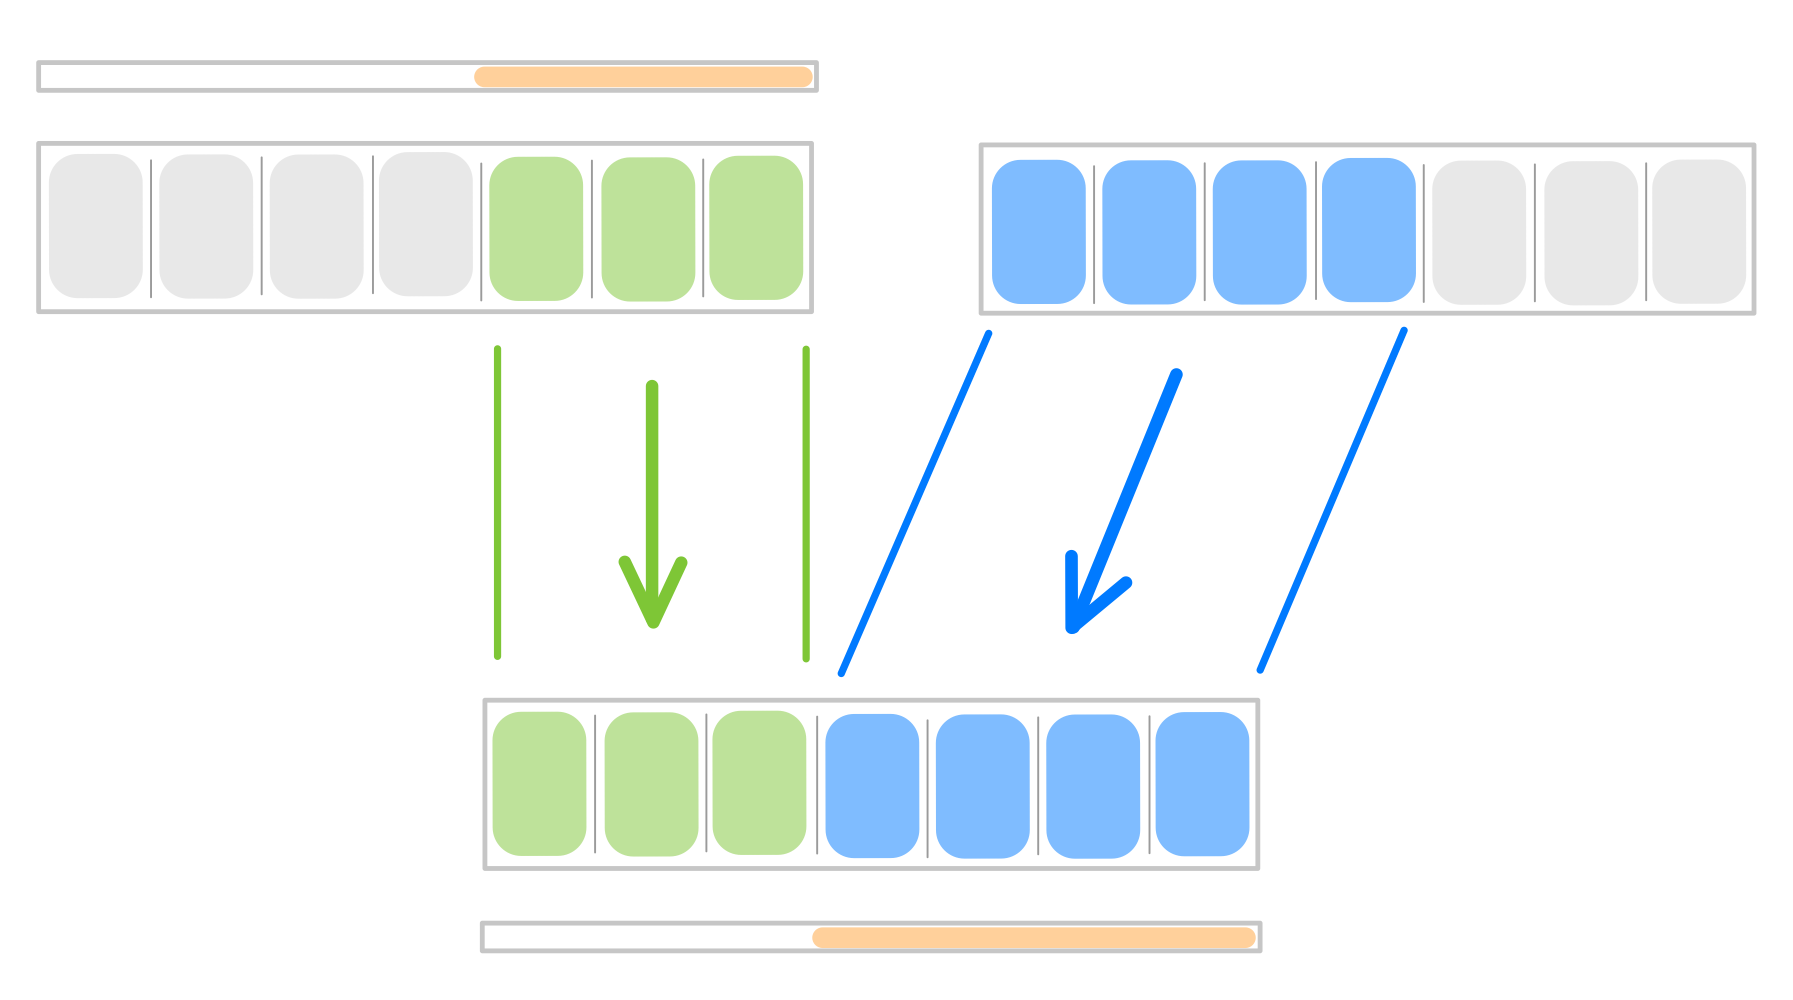
\includegraphics[width = \textwidth]{drawing/2_to_1_full}
\label{fig: one full to two}
\caption{Representation of the surgical pattern implemented by $\twoToOneFull{}$.}
\end{figure}
\fi
